\documentclass[conference]{IEEEtran}
\IEEEoverridecommandlockouts

\usepackage{cite}
\usepackage{amsmath,amssymb,amsfonts}
\usepackage{algorithmic}
\usepackage{graphicx}
\usepackage{textcomp}
\usepackage{xcolor}

\def\BibTeX{{\rm B\kern-.05em{\sc i\kern-.025em b}\kern-.08em
    T\kern-.1667em\lower.7ex\hbox{E}\kern-.125emX}}
    
% A shortcut for µRTS
\newcommand{\mRTS}{$\mu$RTS}

\begin{document}

\title{Enhancing MCTS Performance in Real-Time Strategy Games Through Move Pruning}

\author{
\IEEEauthorblockN{Abdessamed Ouessai\IEEEauthorrefmark{1}, Mohammed Salem\IEEEauthorrefmark{1} and Antonio M. Mora\IEEEauthorrefmark{2}}

\IEEEauthorblockA{\IEEEauthorrefmark{1}Dept. of Computer Sciences, University of Mascara, Algeria.\\
abdessamed.ouessai@univ-mascara.dz, salem@univ-mascara.dz}

\IEEEauthorblockA{\IEEEauthorrefmark{2}Dept. of Signal Theory, Telematics and Communications, ETSIIT-CITIC, University of Granada, Spain.\\
amorag@ugr.es}
}

\maketitle

\begin{abstract}

\end{abstract}

\begin{IEEEkeywords}

\end{IEEEkeywords}

\section{Introduction}

The complexity of real-time strategy (RTS) games, from an AI perspective, originates from the combinatorial structure of their state and decision spaces. In comparison with classic, benchmark games, such as Chess or Go, the dimensionality of both state, and decision spaces in an RTS game is many orders of magnitude higher \cite{ontanon_survey_2013}. Instead of controlling a single unit in a turn-based fashion, as in the previously mentioned board games, RTS players control multiple units simultaneously, in real-time, and usually, in a much larger board (map) size. The branching factor in an RTS game grows exponentially with the increase in the number of units positioned on the map.

Due to the game's complexity, conceiving a human-challenging, RTS game-playing agent is a challenging task to undertake. The predominant approach taken by researchers and practitioners in the domain, is to decompose the task into manageable sub-tasks targeting various degrees of abstraction. Most commonly, an RTS agent combines high-level strategic components, and low-level tactical components \cite{barriga_combining_2017}. Such decomposition is inspired by the way human players interweave micro- and macro-management, and is shown to be effective by numerous implementations.

Holistic, search-based approaches such as MCTS (Monte Carlo Tree Search), enjoyed a remarkable success in computer Go, as demonstrated by AlphaGo \cite{silver_mastering_2016}. However, in RTS games, MCTS-based agents struggle with the enormous decision space, and fail to scale suitably when the branching factor grows past a certain threshold. Such downside, limits MCTS applicability to smaller and limited scenarios, such as tactical planning, or small maps. Abstracting the decision space is a tried and tested technique for scaling MCTS-based approaches to larger scenarios, at the expense of sacrificing tactical performance, due to the coarser actions considered.

In this paper, we propose an approach to enhance the performance and scalability of search-based techniques, particularly MCTS-based, by pruning unnecessary and detrimental player-actions, from the decision space of an RTS game. We inspect the low-level structure of the search space and identify detrimental player-actions, and then apply a number of hard-pruning approaches to remove those player-actions during search. The desired outcomes of such approach is the reduction of the branching factor, and the exploration of more promising player-actions. Our pruning approach focuses on a class of player-actions we identify as Inactive Player-Actions, and is applied using UCT and NaïveMCTS. The experimentation results, using \mRTS{}, show an important performance gain, relative to the size of the map in use.

The rest of this paper is organized as follows : Section II reviews some background information about RTS games, \mRTS{} and MCTS. Section III presents some works related to our approach and Section IV describes Inactive Player-Actions and the move pruning approaches implemented. Experimental results are presented and discussed in Section V, and Section VI concludes the paper with an overall conclusion and some future perspectives.

\section{Background}

\subsection{Real-Time Strategy Games}

A sub-genre of strategy video games, real-time strategy games simulate a warfare situation, where each side of the game is given control over a military base, and is tasked with collecting resources and recruiting troops. To emerge victorious, the player has to completely annihilation the opponent's forces. RTS games progress in real-time, which signifies that players can act simultaneously, and that the effect of executing an action is not necessarily immediate, in addition to the very short decision cycle. Usually, an RTS is played from a top-down perspective, over a large grid-based map, covered by a fog-of-war layer reducing observability, thus, making the game even more difficult. Furthermore, the execution of a player-action can be influenced by some stochastic parameters, introducing non-determinism to the mix. Players control their units by issuing unit-actions to each, and a player-action is the combination of unit-actions issued simultaneously at a given game cycle.

A typical RTS game can is defined as a zero-sum, multi-player, non-deterministic game with incomplete information. The size of an RTS state space and branching factor, as estimated in a typical \textsc{StarCraft} setting \cite{ontanon_survey_2013}, reaches $10^{1685}$ possible states and $10^{50}$ possible actions in a decision point, respectively. In contrast, Chess and Go possess a state space estimate of $10^{47}$, and $10^{171}$ respectively, with a branching factor equalling $36$ in Chess, and $180$ in Go. These estimates are a clear indicator of the difficulty faced by a game-playing AI in the RTS domain, justifying the growing research interest into this domain.

Based on the terminology and definitions presented in \cite{ontanon_combinatorial_2017}, an RTS game can be defined formally as a tuple $G$, where $G = (S, A, P, \tau, L, W, s_{init})$ and each component defined as follows:

\begin{itemize}
\item $S$ : the set of all possible states (state space).
\item $A$ : the set of player-actions (decision space).
\item $P$ : the players set, where $P=\{max,min\}$ for a 2-player setting.
\item $\tau : S \times A \times A \rightarrow S$ : the state transition function, taking a game state in time $t$ and the player-actions of both players, and returns a new game state in $t+1$.
\item $L: S \times A \times P \rightarrow \{true,false\}$ : determines the legality of a player-action in a state for a specific player.
\item $W: S \rightarrow P \cup \{ongoing,draw\}$ : determines the winner of the game (if any) or if the game is a draw or is still ongoing.
\item $s_{init} \in S$ : the initial state.
\end{itemize}

\subsection{\mRTS{}}

Conducting AI research on commercial RTS games was not a smooth experience, as most games did not offer a suitable API for AI research. To mitigate this shortcoming, several independent solutions were developed, such as the unofficial \textsc{StarCraft} interface, BWAPI, the \textsc{WarCraft} port, Wargus and ORTS. Much later, an official API, and tool set for \textsc{StarCraft II} was made available, in a collaborative effort between Blizzard and DeepMind \cite{vinyals_starcraft_2017-1}. Additionally, several independent platforms have emerged such as \mRTS{} \cite{ontanon_combinatorial_2013}, ELF \cite{tian_elf_2017} and DeepRTS \cite{andersen_deep_2018}.

In this paper, we use \mRTS{} as our experimentation test-bed. \mRTS{} is a stripped down RTS game simulator specifically designed for AI research, it features all the challenging aspects of an RTS, without frills. Most importantly, it includes an efficient forward-model, necessary for implementing simulation-based search approaches. A screenshot of a \mRTS{} match is shown in Figure \ref{mRTSScreenshot}. Each player controls 2 types of buildings (Base and Barracks) and 4 types of mobile units (Worker, Light, Ranged, Heavy). The Base is responsible for producing Workers, and the Barracks produces assault units, in exchange with an amount resources. Resources are accumulated in the base by Worker units, which harvest them from resource deposits. A map consists of an arbitrary-sized 2D grid, where each square is either free, or occupied by a unit, a structure, or an environment unit (resource deposit or a wall).

\begin{figure}[t]
\begin{center}
	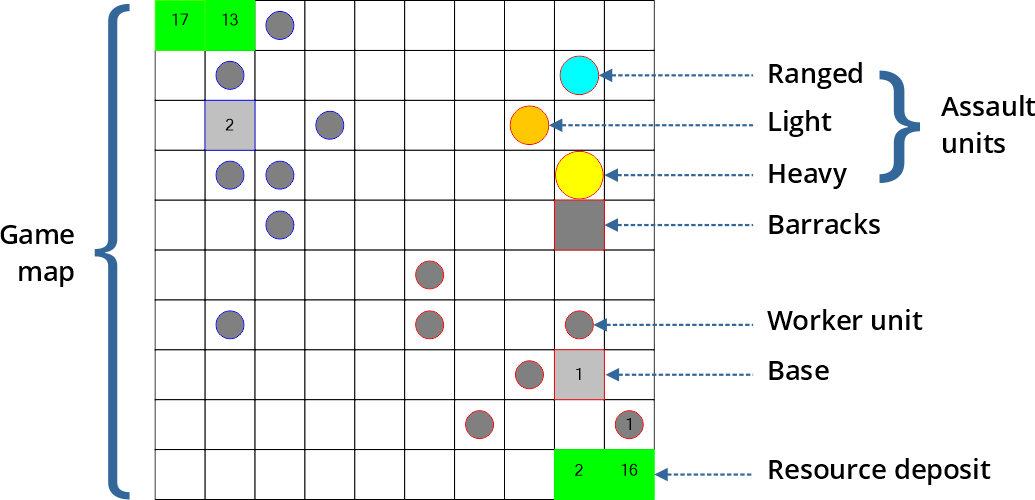
\includegraphics[scale=1]{figs/mRTS.png}
	\caption{A \mRTS{} match. Each player's units can be differentiated by the color of their outline. Blue is for Player 1, and red is for Player 2. The numbers displayed over certain units indicate the amount of resources held by that unit. }
	\label{mRTSScreenshot}
\end{center}
\end{figure}

\mRTS{} represents an interesting research domain for online planning techniques, especially those requiring a forward-model. Several interesting low-level, high-level and hybrid planning approaches were proposed in \mRTS{} as detailed in \cite{ouessai_online_2019}.

\subsection{Monte Carlo Tree Search (MCTS)}

The goal of an RTS game-playing agent is to compute the optimal player-action $a \in A$, for each decision cycle $t$, where the agent is able to act. The successive, computed player-actions constitute a plan that should lead the agent to victory. Essentially, this translates to a Markov decision process (MDP) under tight computation budget, and high search-space dimensionality constraints. MCTS is a sampling-based search framework applicable to MDPs with a large decision space, where systematic search approaches cannot be applied. MCTS relies on the execution of a large number of Monte Carlo simulations to estimate the value of actions, sampled from the search space following a tree-policy. The MCTS algorithm follows a 4-steps iterative process that can be halted anytime to obtain a decision, one MCTS iteration works as follows : 

\begin{enumerate}
\item Selection : Select a node with unexplored children, following a tree policy.
\item Expansion : Expand the selected node by creating and attaching a new child node.
\item Simulation : Start a simulation (playout) from the new node, following a playout policy.
\item Backpropagation : Backpropagate the simulation's results starting from the new node up to the root node.
\end{enumerate}

The game tree is constructed iteratively, and given enough computation budget and a proper exploration / exploitation equilibrium in the tree policy, MCTS is guaranteed to find the minimax solution, in the limits. The most popular MCTS implementation, UCT (Upper Confidence bounds for Trees), uses UCB1 formula as a tree policy, treating the selection phase as a multi-armed bandit (MAB) problem. Although remarkably successful in Go, UCT does not perform as well in RTS games, due to the rapid growth in the branching factor, with the increase in the unit count. NaïveMCTS was specifically designed to address the combinatorial search space in RTS games, by formulating the selection phase as combinatorial MAB (CMAB). Additionaly, NaïveMCTS employs a naïve sampling approach that relies on a naïve assumption considering the reward estimate of a player-action as the sum of the reward estimates of the underlying unit-actions. In our experiments, we used both UCT and NaïveMCTS as the base search algorithms for our pruning approach.

% Writing ...

\section{Related Works}

\section{Move Pruning}

\subsection{Inactive Player-Actions}

\subsection{Pruning Techniques}

\section{Experimentation Results}

\subsection{Parameter Tuning}

% WIP

\begin{figure*}[!h]
\begin{center}
	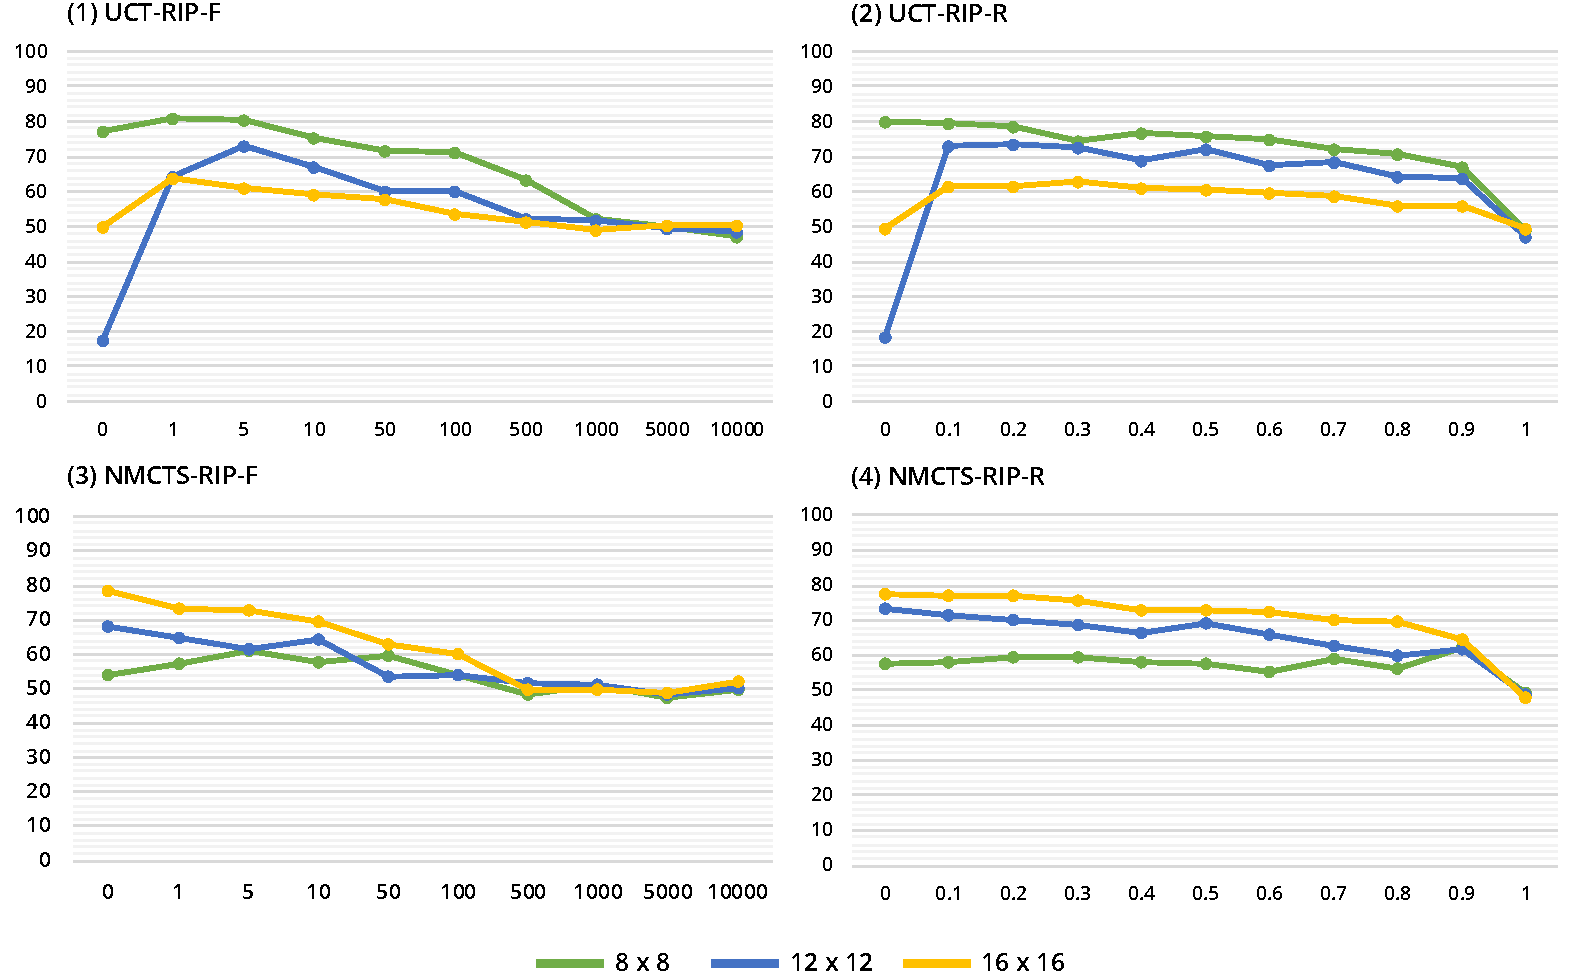
\includegraphics[width=0.8\textwidth]{figs/PT.pdf}
	\caption{UCT-RIP-F performance against UCT}
	\label{PT}
\end{center}
\end{figure*}

\subsection{Best Pruning Approach}

\subsection{Tournament}

\section{Conclusion}

\bibliographystyle{IEEEtranS}
\bibliography{library}

\end{document}
